% --------------| Q01 |--------------------
\addcontentsline{toc}{section}{Problema 01}
\begin{prob}
	Considere a função de onda
	\begin{align}
		\Psi(x,t)&=A \mathrm{e}^{-\lambda |x|} \mathrm{e}^{-i\omega t}
	\end{align}
	onde $A$, $\lambda$ e $\omega$ são constantes reais positivas
	\begin{enumerate}[label=\alph *)]
		\item Normalize $\Psi$
		\item Determine os valores médios $\langle x \rangle$ e $\langle x^{2} \rangle$
		\item Encontre o desvio padrão de $x$. Esboce o gráfico de $|\Psi|^2$ como uma função de $x$, e marque os pontos $\left(\langle x \rangle + \delta \right)$ e $\left(\langle x \rangle - \delta\right)$ para representar em que sentido de $\sigma$ representa o ``espalhamento'' da distribuição em $x$. Qual a probabilidade de que a partícula seja encontrada fora deste range?
	\end{enumerate}

	\begin{sol}
		\begin{enumerate}[label=\alph *)]
			\item Dado que a normalização da função de onda $\Psi (x,t)$ é obtida por  
				\begin{align}
					\int\limits_{-\infty}^{\infty}|\Psi (x,t)\Psi^{*} (x,t)|dx &= \int\limits_{-\infty}^{+\infty}|\psi (x)|^{2}dx = 1
				\end{align}
				de modo que
				\begin{align}
					\int\limits_{-\infty}^{+\infty}|A \mathrm{e}^{-\lambda |x|} \mathrm{e}^{-i \omega t}A \mathrm{e}^{-\lambda |x|} \mathrm{e}^{+i \omega t}|dx &=1 \nonumber\\
					\int\limits_{-\infty}^{+\infty}A^{2} \mathrm{e}^{-2 \lambda |x|}dx &= 1
				\end{align}
				a $\psi(x)$ é uma função par $\psi(x) = \psi(-x)$ e o intervalo de integração é simétrico em $x$, o que nos permite fazer
				\begin{align}
					2A^{2}	\int\limits_{0}^{+\infty} \mathrm{e}^{-2 \lambda |x|}dx &= 1\nonumber \\
					2A^{2}\left(-\frac{1}{2 \lambda} \mathrm{e}^{-2 \lambda x}\bigg|_{0}^{+\infty}\right) &= 1\nonumber \\
					A^{2} &= \lambda \nonumber \\
					A &= \sqrt{\lambda}
				\end{align}
				ou seja
				\begin{dmath*}
					\boxed{
						\Psi(x,t)=\psi(x)\mathrm{e}^{-i \omega t}\condition{com $\displaystyle \psi(x)=\sqrt{\lambda}\mathrm{e}^{-\lambda |x|}$}
					}
				\end{dmath*}
			\item Calculando $\langle x \rangle$ e $\langle x^{2} \rangle$
				\begin{align}
					\begin{split}
						\langle x \rangle &= \int\limits_{- \infty}^{\infty}\abs{\Psi^{*}(x,t)x \Psi(x,t)}\,d{x} = \int\limits_{- \infty}^{\infty}x \abs{\psi(x)}^{2}\,d{x}\\
															&= \int\limits_{- \infty}^{\infty}x \lambda \mathrm{e}^{-2 \lambda x}\,d{x}
					\end{split}
				\end{align}
				neste caso a função $\psi(x)$ é ímpar $\psi(-x)=-\psi(x)$, o que num intervalo de integração simétrico com relação a origem, retorna zero, ou seja
				\begin{align}
					\boxed{
						\langle x \rangle = 0
					}						
				\end{align}
				Para $\langle x^{2} \rangle$, tem-se que
				\begin{align}
					\begin{split}
						\langle x^{2} \rangle &= \int\limits_{- \infty}^{\infty}x^{2}\abs{\psi(x)}^{2}\,d{x}\\
																	&=\lambda \int\limits_{- \infty}^{\infty}x^{2}\mathrm{e}^{-2 \lambda x}\,d{x}
					\end{split}
				\end{align}
				$\psi(x)$ é novamente par, então
				\begin{align}
					\langle x^{2} \rangle &= 2 \lambda \int\limits_{0}^{\infty}x^{2}\mathrm{e}^{-2 \lambda x}\,d{x}\\
				\end{align}
				usando integração por partes duas vezes, chegamos ao seguinte resultado
				\begin{align}
					\begin{split}
						\langle x^{2} \rangle &= -\left[\frac{x^{2}}{\mathrm{e}^{2 \lambda x}}\Bigg|_{0}^{\infty}+\frac{x}{\lambda \mathrm{e}^{2 \lambda x}}\Bigg|_{0}^{\infty}+\frac{2}{2 \lambda \mathrm{e}^{2 \lambda x}}\Bigg|_{0}^{\infty}\right]\implies \left[-\frac{\infty}{\infty}\right]\\
																	&= -\lim_{x\to \infty}\frac{x^{2}}{\mathrm{e}^{2 \lambda x}} \implies \left[-\frac{\infty}{\infty}\right]\\
						\overset{\mathrm{H}}&{=} -\lim_{x\to \infty}\frac{2x}{2 \lambda \mathrm{e}^{2 \lambda x}}\implies \left[-\frac{\infty}{\infty}\right]\\
						\overset{\mathrm{H}}&{=} -\lim_{x\to \infty}\frac{2}{4 \lambda^{2}\mathrm{e}^{2 \lambda x}}\implies \left[0\right]\therefore\\
																&= -\left[\lim_{b\to \infty}\frac{2}{4 \lambda^{2} \mathrm{e}^{2 \lambda x}}\Bigg|_{0}^{b} \right]\\
																&= -\left(0-\frac{1}{2 \lambda^{2}}\right)
					\end{split}
				\end{align}
				\begin{align}
					\boxed{
						\langle x^{2} \rangle = \frac{1}{2 \lambda^{2}}
					}
				\end{align}
			\item Calculando $\sigma$
				\begin{align}
					\begin{split}
						\sigma &= \sqrt{\langle x^{2} \rangle-\langle x \rangle^{2}}\\
									 &= \sqrt{\frac{1}{2 \lambda^{2}}-0}\\
									 &= \frac{1}{\lambda\sqrt{2}}
					\end{split}						
				\end{align}
				\begin{align}
					\boxed{\sigma = \frac{\sqrt{2}}{2\lambda}}
				\end{align}
				\begin{figure}[ht!]
					\centering
					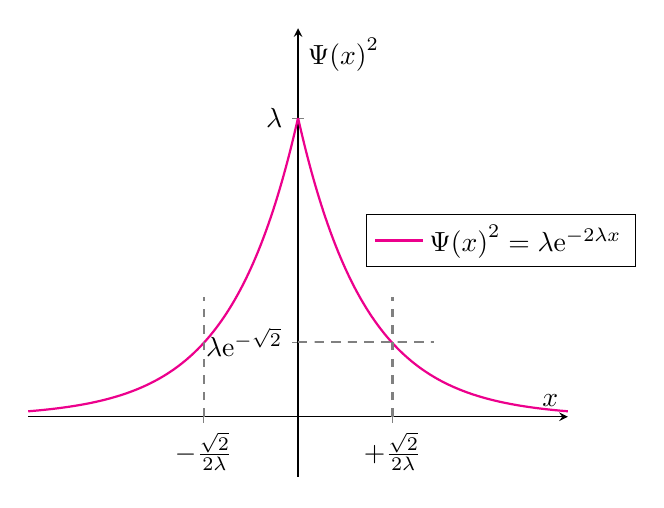
\begin{tikzpicture}[scale=1] 
  \begin{axis}[
	 axis lines = center,                
	 xmin = -2, xmax = 2,
	 ymin = -0.2, ymax = 1.3,
	 xlabel = {$x$},
	 ylabel = {$\abs{\Psi(x)}^{2}$},
	 ytick = {0.25, 1},
	 yticklabels = {$\lambda \mathrm{e}^{-\sqrt{2}}$,$\lambda$},
	 xtick = {-0.7, 0.7},
	 xticklabels = {$-\frac{\sqrt{2}}{2 \lambda}$, $+\frac{\sqrt{2}}{2 \lambda}$},
	 % legend pos = south west,
	 legend style={at={(axis cs:0.5,0.5)},anchor=south west},
	 ]
	 \addplot[
	 domain = -2:2,
	 samples = 1000,
	 smooth,
	 thick,
	 magenta,
	 ] {exp(-2*abs(x))};                
	 \addlegendentry{$\abs{\Psi(x)}^{2}=\lambda\mathrm{e}^{-2 \lambda \abs{x}}$}
	 \addplot[
	 domain = 0:1,
	 samples = 1000,
	 dashed,
	 thick,
	 gray,
	 ] {0.25};
	 %% This is the vertical line
	 \addplot[thick,dashed,domain=-2:2,gray] coordinates {(0.7,0)(0.7,0.4)};
	 \addplot[thick,dashed,domain=-2:2,gray] coordinates {(-0.7,0)(-0.7,0.4)};
  \end{axis}         
	% \draw [dashed] (2.9,.6) -- (2.9, 2);
\end{tikzpicture}  

					\caption{Região de probabilidade de encontrar a partícula entre os valores do desvio padrão $\pm\sigma$}
					\label{fig:pltQ01c}
				\end{figure}
				Para valores de $x\in (-\infty, -\sigma]$ e $x\in [+\sigma,+\infty)$, tem-se que
				\begin{align}
					\begin{split}
						2 \lambda \int\limits_{\sigma}^{\infty}\mathrm{e}^{-2 \lambda\abs{x}}\,d{x} &= 2 \lambda \left[-\frac{1}{2 \lambda}\mathrm{e}^{-2 \lambda x}\Bigg|_{\sigma}^{\infty} \right]\\
																																												&= 0+\frac{1}{\mathrm{e}^{2 \lambda \sigma}}\\
																																												&= \frac{1}{\mathrm{e}^{\sqrt{2}}}
					\end{split}
				\end{align}
		\end{enumerate} 	
	\end{sol}
\end{prob}

%--------------| Q02 |--------------------
\addcontentsline{toc}{section}{Problema 02}
\begin{prob}
	O Teorema de Ehrenfest
	\begin{enumerate}[label=\alph *)]
		\item Mostre que, para uma função de $x$ qualquer, vale a seguinte relação de comutação:
			\begin{align}
				\left[\hat{p},f(x)\right] &= -i\hbar \frac{\partial f(x)}{\partial x}
			\end{align}
		\item Utilize o resultado do item (a), o fato que o operador momento comuta com funções apenas do momento e a evolução temporal do valor médio dos operadores
			\begin{align}
				\frac{d \langle Q \rangle}{dt} &= \frac{1}{i \hbar} \Bigl\langle \left[\hat{Q}, \hat{H}\right] \Bigr\rangle
			\end{align}
			e obtenha o Teorema de Ehrenfest
	\end{enumerate}

	\begin{sol}
		\begin{enumerate}[label=\alph *)]
			\item	Façamos o comutador atuar em uma função $\psi (x)$, de modo que
				\begin{align}
					\left[\hat{p},f(x)\right] \psi(x) &= \hat{p}f(x) \psi(x)-f(x)\hat{p} \psi(x)\nonumber\\
																						&= -i \hbar \frac{\partial }{\partial x}\left[f(x) \psi(x)\right]+i \hbar f(x) \frac{\partial \psi(x)}{\partial x}\nonumber \\
																						&= \left(-i \hbar\right)\left[\frac{\partial f(x)}{\partial x} \psi(x)+f(x)\frac{\partial \psi(x)}{\partial x}-f(x)\frac{\partial \psi(x)}{\partial x}\right]\nonumber\\
																						&= -i \hbar \frac{\partial f(x)}{\partial x} \psi(x)
				\end{align}
				o que resulta em
				\begin{align}
					\boxed{
						\left[\hat{p},f(x)\right] = -i \hbar \frac{\partial f(x)}{\partial x}
					}
				\end{align}\qed

			\item Dado que
				\begin{align}
					\frac{d \langle Q \rangle}{dt} &= \frac{1}{i \hbar} \Bigl \langle \left[\hat{Q},\hat{H}\right] \Bigr \rangle\nonumber\\
																				 &= \frac{1}{i \hbar} \int\limits_{-\infty}^{\infty} \psi^{*}\left[\hat{Q},\hat{H}\right] \psi dx
				\end{align}
				ou seja
				\begin{align}
					\frac{d \langle Q \rangle}{dt} &= \frac{1}{i \hbar} \int\limits_{-\infty}^{\infty} \psi^{*}\left(\hat{Q}\hat{H}-\hat{H}\hat{Q}\right) \psi dx\nonumber\\
																				 &= \frac{1}{i \hbar} \int\limits_{-\infty}^{\infty} \psi^{*}\hat{Q}\hat{H} \psi dx-\frac{1}{i \hbar}\int\limits_{-\infty}^{\infty} \psi^{*}\hat{H}\hat{Q} \psi dx\nonumber\\
																				 &= \frac{1}{i \hbar} \int\limits_{-\infty}^{\infty} \psi^{*}\hat{Q}\left(\frac{\hat{p}^{2}}{2m}+V\right) \psi dx-\frac{1}{i \hbar}\int\limits_{-\infty}^{\infty} \psi^{*}\left(\frac{\hat{p}^{2}}{2m}+V\right)\hat{Q} \psi dx\nonumber\\
																				 &= \frac{1}{i \hbar}\left[\frac{1}{2m}\left(\int\limits_{-\infty}^{\infty} \psi^{*}\hat{Q}\hat{p}^{2} \psi dx-\int\limits_{-\infty}^{\infty} \psi^{*}\hat{p}^{2}\hat{Q} \psi dx\right)+\right.\nonumber\\&\left.\qquad +\int\limits_{-\infty}^{\infty} \psi^{*}\hat{Q}V \psi dx-\int\limits_{-\infty}^{\infty} \psi^{*}V \hat{Q} \psi dx\right]\nonumber\\
																				 &= \frac{1}{2i \hbar m}\int\limits_{-\infty}^{\infty}\left(\psi^{*}\hat{Q}\hat{p}^{2} \psi-\psi^{*}\hat{p}^{2}\hat{Q} \psi\right)dx+\nonumber\\&\qquad +\frac{1}{i \hbar}\int\limits_{-\infty}^{\infty}\left(\psi^{*}\hat{Q}V \psi-\psi^{*}V \hat{Q} \psi\right)dx\nonumber\\
																				 &= \frac{1}{2i \hbar m}\Bigl \langle \left[\hat{Q},\hat{p}^{2}\right] \Bigr \rangle+\frac{1}{i \hbar}\Bigl \langle \left[\hat{Q},V\right] \Bigr \rangle
				\end{align}
				Agora, desde que $\hat{Q}$ possa ser escrito como $\hat{Q}=\hat{p}$, devemos ter
				\begin{align}
					\frac{d \langle p \rangle}{dt}&= \frac{1}{2i \hbar m}\Bigl \langle \left[\hat{p},\hat{p}^{2}\right] \Bigr \rangle+\frac{1}{i \hbar}\Bigl \langle \left[\hat{p},V\right] \Bigr \rangle
				\end{align}
				se o operador $\hat{p}$ comuta com funções do momento então $\left[\hat{p},\hat{p}^{2}\right]=0$, além do mais se $V=V(x)$, já vimos que
				\begin{align}
					\left[\hat{p},V(x)\right] &= -i \hbar \frac{\partial V(x)}{\partial x}
				\end{align}
				e portanto,
				\begin{align}
					\frac{d \langle p \rangle}{dt} &= \frac{1}{i \hbar} \Bigl \langle [\hat{p}, V] \Bigr \rangle\nonumber\\
					\frac{d \langle p \rangle}{dt} &= \Bigl \langle -\frac{\partial V}{\partial x} \Bigr \rangle \nonumber\\
				\end{align}
				\begin{align}
					\boxed{
						\frac{d \langle p \rangle}{dt} = -\Bigl \langle \nabla V \Bigr \rangle
					}
				\end{align}\qed
		\end{enumerate}
	\end{sol}
\end{prob}

%--------------| Q03 |--------------------
\addcontentsline{toc}{section}{Problema 03}
\begin{prob}
	Em aula resolvemos o problema do poço infinito com centro deslocado da origem. Resolva o poço infinito para o caso onde o centro do poço coincide com a origem, isto é:	

	\begin{eqnarray*}
		V(x)=
		\begin{cases}
			\infty, &\text{se $x < -a/2$}\\
			0, &\text{se $-a/2\leq x\leq a/2$}\\
			\infty, &\text{se $x > a/2$}\\
		\end{cases}
	\end{eqnarray*}

	\begin{center}
		\tikzset{every picture/.style={line width=0.75pt}} %set default line width to 0.75pt        
		\begin{tikzpicture}[x=0.75pt,y=0.75pt,yscale=-1,xscale=1]
			%uncomment if require: \path (0,619); %set diagram left start at 0, and has height of 619
			%Straight Lines [id:da6357675944815533] 
			\draw    (160,507) -- (354,507) ;
			\draw [shift={(356,507)}, rotate = 180] [color={rgb, 255:red, 0; green, 0; blue, 0 }  ][line width=0.75]    (10.93,-3.29) .. controls (6.95,-1.4) and (3.31,-0.3) .. (0,0) .. controls (3.31,0.3) and (6.95,1.4) .. (10.93,3.29)   ;
			%Straight Lines [id:da7577447653081695] 
			\draw    (248,507.5) -- (248,376.5) ;
			\draw [shift={(248,374.5)}, rotate = 90] [color={rgb, 255:red, 0; green, 0; blue, 0 }  ][line width=0.75]    (10.93,-3.29) .. controls (6.95,-1.4) and (3.31,-0.3) .. (0,0) .. controls (3.31,0.3) and (6.95,1.4) .. (10.93,3.29)   ;
			%Straight Lines [id:da6135058394659405] 
			\draw  [dash pattern={on 0.84pt off 2.51pt}]  (287,507) -- (287,484.5) -- (287,418.5) ;
			%Straight Lines [id:da3554258374645527] 
			\draw  [dash pattern={on 0.84pt off 2.51pt}]  (208,507) -- (208,444.61) -- (208,418.5) ;


			% Text Node
			\draw (242,510.49) node [anchor=north west][inner sep=0.75pt]    {$0$};
			% Text Node
			\draw (187,507.18) node [anchor=north west][inner sep=0.75pt]    {$-a/2$};
			% Text Node
			\draw (271,507.18) node [anchor=north west][inner sep=0.75pt]    {$a/2$};
			% Text Node
			\draw (363,500.18) node [anchor=north west][inner sep=0.75pt]    {$x$};
			% Text Node
			\draw (233,343.18) node [anchor=north west][inner sep=0.75pt]    {$V( x)$};
		\end{tikzpicture}
	\end{center}
	Para este problema encontre as autofunções $\psi_{n}(x)$ e os autovalores de energia $E_{n}$.
	\begin{sol}
		A equação de Schrödinger para pontos no interior do poço é dada por
		\begin{align}
			\frac{-\hbar^{2}}{2m}\frac{\partial^{2} \psi(x)}{\partial x^{2}} &= E \psi(x)
			\label{eq:sch-symPotential}
		\end{align}
		manipulando a equação \eqref{eq:sch-symPotential} obtemos
		\begin{align}
			\begin{split}
				\frac{\partial^{2} \psi(x)}{\partial x^{2}} &= -\frac{2mE}{\hbar^{2}} \psi(x)\\
				\frac{\partial^{2} \psi(x)}{\partial x^{2}} &= -k^{2} \psi(x)\\
			\end{split}
		\end{align}
		cujo a solução geral é dada por
		\begin{dmath*}
			\psi(x)A\sen(kx)+B\cos(kx)\condition{com $\displaystyle k=\sqrt{\frac{2mE}{\hbar^{2}}}$}
		\end{dmath*}
		da condição de contorno sabemos que
		\begin{subequations}
			\begin{align}
				\psi(a/2)=A\sen(ka/2)+B\cos(ka/2) &=0 \label{eq:sch-symPotential-CCa}\\
				\psi(-a/2)=A\sen(-ka/2)+B\cos(-ka/2) &= 0\label{eq:sch-symPotential-CCb}
			\end{align}
		\end{subequations}
		O par de equações descrito pelas \eqref{eq:sch-symPotential-CCa} e \eqref{eq:sch-symPotential-CCb}, formam um sistema de equações. A função \textit{seno} é uma função \textit{ímpar} o que equivale a dizer que $\sen(-x)=-\sen(x)$, já a função \textit{cosseno} é uma função \textit{par} isto é $\cos(-x)=\cos(x)$, logo
		\begin{align}
			\begin{split}
				A\sen(ka/2)+B\cos(ka/2) &= 0\\
				-A\sen(ka/2)+B\cos(ka/2) &= 0
			\end{split}				
		\end{align}
		resolvendo o sistema para o \textit{cosseno}, obtemos
		\begin{align}
			2B\cos(ka/2) &= 0
		\end{align}
		$B$ não pode ser nulo, do contrário não há função de onda no intervalo de interesse, portanto
		\begin{align}
			\cos \left(\frac{ka}{2}\right) &= 0 \iff \frac{ka}{2}=\frac{\pi}{2},\frac{3 \pi}{2},\frac{5 \pi}{2},\ldots 
		\end{align}
		por outro lado, se resolvermos o sistema para o \textit{seno}, teremos
		\begin{align}
			2A\sen(ka/2) &= 0
		\end{align}
		tal como anteriormente $A$ é não nulo de modo que
		\begin{align}
			\sen \left(\frac{ka}{2}\right) &= 0 \iff \frac{ka}{2}=\pi,2 \pi,3 \pi,\ldots
		\end{align}
		Há portanto duas soluções possíveis para a $\psi(x)$
		\begin{align}
			\psi_{n}(x)=
			\begin{dcases*}
				A_{n}\sen \left(k_nx\right) & se, $n=2, 4, 6,...$(par)\\
				B_{n}\cos \left(k_nx\right) & se, $n=1, 3, 5, ...$(ímpar)\\
			\end{dcases*}
		\end{align}
		e
		\begin{align}
			k_{n} &= \frac{n \pi}{a}
		\end{align}
		As constantes $A_{n}$ e $B_{n}$ são obtidas impondo a condição de normalização das funções $\psi(x)$
		\begin{align}
			\int\limits_{-\infty}^{\infty} |\psi^{*}_{n}(x) \psi_{n}(x)|^{2}dx &= \int\limits_{-\infty}^{\infty}|\psi_{n}(x)|^{2}dx=1\\
		\end{align}
		para $n=2, 4, 6,...$
		\begin{align}
			\begin{split}
				\int\limits_{-\infty}^{-\frac{a}{2}}|\cancelto{0}{\psi_{n}(x)}|^{2}dx+\int\limits_{-\frac{a}{2}}^{\frac{a}{2}}|\psi_{n}(x)|^{2}dx+\int\limits_{\frac{a}{2}}^{\infty}|\cancelto{0}{\psi_{n}(x)}|^{2}dx &= 1\\
				\int\limits_{-\frac{a}{2}}^{\frac{a}{2}}A^{2}_{n}\sen^{2} \left(\frac{n \pi x}{a}\right)dx &= 1\\
				A^{2}_{n}\int\limits_{-\frac{a}{2}}^{\frac{a}{2}}\sen^{2}\left(\frac{n \pi x}{a}\right)dx &= 1\\
			\end{split}
		\end{align}
		fazendo a mudança de variável $u=n \pi x/2$, $du=n \pi dx/2$, quando $x=-\pi/2$ então $u=-n \pi /2$, e quando $x=\pi/2$, $u=n \pi/2$, dessa forma o resultado da integral acima fica
		\begin{align}
			\begin{split}
				A^{2}_{n}\left[\frac{a}{n \pi}\right]\left[\left(\frac{n \pi}{2}\right)-\frac{1}{2}\cancelto{0}{\left(\frac{\sin(2u)}{2}\right)\Bigg|_{-n \pi/2}^{n \pi/2}}\right] &= 1
			\end{split}
		\end{align}
		o que simplificando da
		\begin{align}
			A_{n} &= \sqrt{\frac{2}{a}}
		\end{align}
		A solução para $n=1,3,5,...$ é similar, mas agora a função que devemos integrar é
		\begin{align}
			B_{n}^{2}\int\limits_{-\frac{a}{2}}^{\frac{a}{2}}\cos^{2} \left(\frac{n \pi x}{a}\right)dx &= 1
		\end{align}
		procedendo de forma análoga obtemos
		\begin{align}
			B^{2}_{n}\left[\frac{a}{n \pi}\right]\left[\left(\frac{n \pi}{2}\right)+\frac{1}{2}\cancelto{0}{\left(\frac{\sin(2u)}{2}\right)\Bigg|_{-n \pi/2}^{n \pi/2}}\right] &= 1
		\end{align}
		ou seja
		\begin{align}
			B_{n} &= \sqrt{\frac{2}{a}}
		\end{align}
		completando a solução para as autofunções $\psi_{n}(x)$
		\begin{align}
			\boxed{
				\psi_{n}(x)=
				\begin{dcases*}
					\sqrt{\frac{2}{a}}\sen \left(\frac{n \pi x}{a}\right) & se, $n=2, 4, 6,...$(par)\\
					\sqrt{\frac{2}{a}}\cos \left(\frac{n \pi x}{a}\right) & se, $n=1, 3, 5, ...$(ímpar)\\
				\end{dcases*}
			}
		\end{align}
		e
		\begin{align}
			\boxed{
				k_{n} = \frac{n \pi}{a}
			}
		\end{align}

		É de se esperar que os autovalores de energia associados $E_{n}$, sejam os mesmos encontrados para o poço infinito com centro deslocado da origem, e de fato, em termos dos $k_{n}$, teremos
		\begin{align}
			\begin{split}
				k_{n} &= \frac{n \pi}{a}=\sqrt{\frac{2mE_{n}}{\hbar^{2}}}\\
			\end{split}
		\end{align}
		\begin{align}
			\boxed{
				E_{n} = \frac{\pi^{2}\hbar^{2}}{2ma^{2}}n^{2}
			}
		\end{align}
	\end{sol}
\end{prob}
% --------------------------------------------- %
% --------------| Q04 |------------------------ %
\addcontentsline{toc}{section}{Problema 04}
\begin{prob}
	Para o problema do poço quadrado infinito calculado em aula (poço assimétrico em torno da origem), calcule $\langle x \rangle$, $\langle x^{2} \rangle$, $\langle p \rangle$ e $\langle p^{2} \rangle$ e use-os para calcular as incertezas $\sigma_{x}$ e $\sigma_{p}$ para o n-ésimo estado estacionário do poço infinito. Mostre que o princípio de incerteza está sendo satisfeito. qual estado $n$ fica mais próximo do limite inferior do princípio de incerteza?
	\begin{sol}
		A solução da parte espacial da função de onda encontrada em aula é a seguinte
		\begin{dmath*}
			\psi_{n}(x) = \sqrt{\frac{2}{a}}\sen \left(\frac{n \pi x}{a}\right)\condition{com $n\in \mathbb{N^{*}},\; 0\leq x\leq a$}
		\end{dmath*}
		logo, teremos
		\begin{align}
			\begin{split}
				\langle x \rangle &= \int\limits_{0}^{a} \psi^{*}x \psi dx\\
													&= \int\limits_{0}^{a}x \abs{\psi}^{2}dx\\
													&= \int\limits_{0}^{a}x \left[\sqrt{\frac{2}{a}}\sen \left(\frac{n \pi x}{a}\right)\right]^{2}dx\\
													&= \frac{2}{a}\int\limits_{0}^{a}x\sen^{2} \left(\frac{n \pi x}{a}\right)dx\\
			\end{split}
		\end{align}
		fazendo a substituição
		\begin{subequations}
			\begin{align}
				u &= \frac{n \pi x}{a}\\
				du &= \frac{n \pi}{a} dx
			\end{align}
		\end{subequations}
		e notando que
		\begin{subequations}
			\begin{align}
				x\to 0 &\implies u\to 0\\
				x\to a &\implies u\to n \pi
			\end{align}
		\end{subequations}
		ajustamos o argumento do \emph{seno} para poder aplicar integração por partes e ficamos com
		\begin{equation*}
			\begin{split}
				\langle x \rangle &= \frac{2}{a}\int\limits_{0}^{n \pi}\left(\frac{a}{n \pi}\right)u\sen^{2}u\left(\frac{a}{n \pi}\right)\,du\\
													&=\frac{2}{a}\left(\frac{a}{n \pi}\right)^{2}\int\limits_{0}^{n \pi}u\sin^{2}{u}\,du
			\end{split}
		\end{equation*}
		no exercício anterior já mostramos que o resultado da integral de $\sin^{2}(x)$, a menos de uma constante, é igual a
		\begin{align}
			\int \sin^{2}x\,dx &= \frac{1}{2}\left[x-\frac{1}{2}\sin(2x)\right] 
		\end{align}
		de modo que, aplicando a integração por partes na integral de interesse, obtemos
		\begin{align}
			\begin{split}
				\frac{2a}{n^{2} \pi^{2}}\int\limits_{0}^{n \pi}u\sin^{2}u\,d{u} &= \frac{2a}{n^{2} \pi^{2}}\left\{\frac{u}{2}\left[u-\frac{1}{2}\sin(2u)\right]\Bigg|_{0}^{n \pi}\right\}-\frac{2a}{n^{2} \pi^{2}}\frac{1}{2}\int\limits_{0}^{n \pi}\left[u-\frac{1}{2}\sin(2u)\right]\,d{u}\\
																																				&= \frac{2a}{n^{2} \pi^{2}}\left[\frac{u^{2}}{2}-\frac{u}{4}\sin(2u)\right]\Bigg|_{0}^{n \pi}-\frac{2a}{n^{2} \pi^{2}}\frac{1}{2}\left[\frac{u^{2}}{2}+\frac{1}{4}\cos(2u)\right]\Bigg|_{0}^{n \pi}\\
																																				&= \frac{2a}{n^{2} \pi^{2}}\left[\frac{n^{2}{\pi^{2}}}{2}-\frac{n \pi}{4}\sin(2n \pi)-\frac{n^{2} \pi^{2}}{4}-\frac{1}{8}\cos(2n \pi)+\frac{1}{8}\right]=\langle x \rangle
			\end{split}
		\end{align}
		Desde que $n\in \mathbb{N^{*}}\implies \sin(2n \pi)=0$ e $\cos(2n \pi)=1$ ou seja
		\begin{align}
			\begin{split}
				\langle x \rangle &= \frac{2a}{n^{2} \pi^{2}}\left[\frac{n^{2} \pi^{2}}{2}-\frac{n^{2} \pi^{2}}{4}\right]=\frac{2a}{n^{2} \pi^{2}}\left(\frac{n^{2} \pi^{2}}{4}\right)\therefore
			\end{split}
		\end{align}
		\begin{align}
			\boxed{
				\langle x \rangle = \frac{a}{2}
			}
		\end{align}
		procedendo de forma análoga para $\langle x^{2} \rangle$
		\begin{align}
			\begin{split}
				\langle x^{2} \rangle	&= \int\limits_{0}^{a}\frac{2}{a}x^{2}\sin^{2}\left(\frac{n \pi x}{a}\right)\,d{x}\\
															&= \frac{2}{a}\int\limits_{0}^{n \pi}\left(\frac{a}{n \pi}\right)^{2}u^{2}\sin^{2}u \left(\frac{a}{n \pi}\right)\,d{u}\\
															&= \frac{2}{a}\left(\frac{a}{n \pi}\right)^{3}\int\limits_{0}^{n \pi}u^{2}\sin^{2}u\,d{u}\\
															&= \frac{2a^{2}}{n^{3} \pi^{3}}\left[\frac{u^{3}}{6}-\frac{u^{2}}{4}\sin{(2u)}-\frac{x}{4}\cos{(2u)}+\frac{1}{8}\sin{(2u)}\right]\Bigg|_{0}^{n \pi}\\
															&= \frac{2a^{2}}{n^{3} \pi^{3}}\left[\frac{n^{3} \pi^{3}}{6}-\frac{n^{2} \pi^{2}}{4}\underbrace{\sin(2n \pi)}_{\displaystyle 0}-\frac{n \pi}{4}\underbrace{\cos{(2n \pi)}}_{\displaystyle 1}+\frac{1}{8}\underbrace{\sin{(2n \pi)}}_{\displaystyle 0}\right]\\
															&= \frac{2a^{2}}{n^{3} \pi^{3}}\left[\frac{n^{3} \pi^{3}}{6}-\frac{n \pi}{4}\right]
			\end{split}
		\end{align}
		portanto,
		\begin{align}
			\boxed{
				\langle x^{2} \rangle = \frac{a^{2}}{3}-\frac{1}{2}\left(\frac{a}{n \pi}\right)^{2}
			}
		\end{align}

		Para determinar $\langle p \rangle$, uma vez que conhecemos $\langle x \rangle$, basta fazermos 
		\begin{align}
			\langle p \rangle &= \frac{d \langle x \rangle}{dt}
		\end{align}
		logo
		\begin{align}
			\langle p \rangle =\frac{d}{dt}\left(\frac{a}{2}\right)
		\end{align}
		ou simplesmente
		\begin{align}
			\boxed{\langle p \rangle=0}
		\end{align}
		Porém para determinar $\langle p^{2} \rangle$, precisaremos da equação de Schröedinger escrita para o problema. Notando que a partícula somente pode exisitir no interior do poço infinito onde a função de onda $\psi(x)$ é diferente de zero, e que nesta região a partícula é livre ($V=0$)
		\begin{align}
			\begin{split}
				\hat{H} \psi &= E\psi\\
				-\frac{\hbar^{2}}{2m}\frac{d^{2}\psi_{n}(x)}{dx^{2}} &= E_{n} \psi_{n}(x)\\
				\frac{d^{2} \psi_{n}(x)}{dx^{2}} &= -\frac{2mE_{n}}{\hbar^{2}} \psi_{n}(x)
			\end{split}
		\end{align}
		atento a isto, segue que
		\begin{align}
			\begin{split}
				\langle p^{2} \rangle &= \int\limits_{0}^{a} \psi_{n}^{*}(x)\left(-i \hbar \frac{d}{dx}\right)^{2} \psi_{n}(x)\,d{x}\\
															&= -\hbar^{2}\int\limits_{a}^{b} \psi^{*}(x)\frac{d^{2} \psi_{n}(x)}{dx^{2}}\,d{x}\\
															&= \hbar^{2}\frac{2mE_{n}}{\hbar^{2}}\int\limits_{0}^{a} \psi_{n}^{*}(x) \psi_{n}(x)\,d{x}
			\end{split}
		\end{align}
		usando a condição de normalização das funções $\psi_{n}(x)$
		\begin{align}
			\langle p^{2} \rangle	&= 2mE_{n}
		\end{align}
		em sala de aula, encontramos para o valor de energia
		\begin{align}
			E_{n} &= \frac{n^{2} \pi^{2} \hbar^{2}}{2ma^{2}}
		\end{align}
		então
		\begin{align}
			\boxed{
				\langle p^{2} \rangle = \left(\frac{n \pi \hbar}{a}\right)^{2}
			}
		\end{align}

		Para o n-ésimo estado estacionário a incerteza na posição é dada por	
		\begin{align}
			\sigma_{x}=\sqrt{\langle x^{2} \rangle -\langle x \rangle^{2}}
		\end{align}
		portanto	
		\begin{align}
			\begin{split}
				\sigma_{x} &= \sqrt{\left[\frac{a^{2}}{3}-\frac{1}{2}\left(\frac{a}{n \pi}\right)^{2}\right]-\frac{a^{2}}{4}}\\
									 &= \sqrt{\frac{a^{2}}{12}-\frac{a^{2}}{2n^{2} \pi^{2}}}\\
			\end{split}
		\end{align}
		\begin{align}
			\boxed{
				\sigma_{x} = \frac{a}{2}\sqrt{\frac{1}{3}-\frac{2}{n^{2} \pi^{2}}}
			}
		\end{align}
		e para o momento teremos
		\begin{align}
			\begin{split}
				\sigma_{p} &= \sqrt{\langle p^{2} \rangle-\langle p \rangle^{2}}\\
									 &= \sqrt{\left(\frac{n \pi \hbar}{a}\right)^{2}}
			\end{split}
		\end{align}
		\begin{align}
			\begin{split}
				\boxed{
					\sigma_{p} = \frac{n \pi \hbar}{a}
				}
			\end{split}				
		\end{align}
		Segundo o princípio de incerteza, não é possível obter simultâneamente com precisão o valor de duas variáveis conjugadas, matemáticamente isso é expresso por
		\begin{align}
			\sigma_{x} \sigma_{p}\geq \frac{\hbar}{2}
		\end{align}
		se isso for verdade, então, para o caso em questão teremos
		\begin{align}
			\begin{split}
				\sigma_{x} \sigma_{p} = \left(\frac{n \pi \hbar}{a}\right)\frac{a}{2}\sqrt{\frac{1}{3}-\frac{2}{n^{2} \pi^{2}}}\\
				= \frac{n \pi \hbar}{2}\sqrt{\frac{1}{3}-\frac{2}{n^{2} \pi^{2}}}\\
			\end{split}
		\end{align}
		usando o princípio de incerteza
		\begin{align}
			\begin{split}
				\sigma_{x} \sigma_{x} &\geq \frac{\hbar}{2}\\
				\frac{n \pi \hbar}{2}\sqrt{\frac{1}{3}-\frac{2}{n^{2} \pi^{2}}}&\geq \frac{\hbar}{2}\\
				n^{2} \pi^{2}\left(\frac{1}{3}-\frac{2}{n^{2} \pi^{2}}\right)&\geq 1\\
				\frac{n^{2} \pi^{2}}{3}-2&\geq 1\\
				\frac{n^{2} \pi^{2}}{3}&\geq 3\\
				n&\geq \frac{3}{\pi}
			\end{split}
		\end{align}
		como $n\in\mathbb{N^{*}}$ a desigualdade acima é sempre verdade, o que de fato satisfaz o princípio de incerteza. O produto $\sigma_{x} \sigma_{p}$ é proporcional a constante reduzida de planck $\hbar$, no intervalo avaliado o menor valor possível de $n$ é $n=1$ o que consequentemente é também o valor mais próximo do limite inferior de incerteza.


	\end{sol}
\end{prob}
% --------------------------------------------- %
% --------------| Q05 |------------------------ %
\addcontentsline{toc}{section}{Problema 05}
\begin{prob}
	Uma partícula num poço quadrado infinito tem como função de onda inicial
	\begin{eqnarray*}
		\Psi(x,0)=
		\begin{cases}
			Ax, &\text{se $0\leq x \leq \frac{a}{2}$}\\
			A \left(a-x\right), &\text{se $\frac{a}{2}\leq x\leq a$}\\
		\end{cases}
	\end{eqnarray*}
	\begin{enumerate}[label=\alph *)]
		\item Esboce o gráfico de $\Psi(x,0)$ e determine a constante de normalização $A$
		\item Encontre $\Psi(x,t)$
		\item Qual é a probabilidade de que uma medida da energia retorne o valor $E_{1}$
		\item Encontre o valor médio da energia
	\end{enumerate}
	\begin{sol}
		\begin{enumerate}[label=\alph *)]
			\item A função $\Psi(x,0)\times x$ encontra-se plotada na Figura \ref{fig:pltQ05a}

				\begin{figure}[ht!]
					\centering
					\begin{tikzpicture}[scale=1]
	\begin{axis}[
		axis lines = center,
		xmin = -.2, xmax=1,
		ymin = -.2, ymax=1,
		]
	\end{axis}
\end{tikzpicture}

					\caption{Gráfico da $\Psi(x,0)$}
					\label{fig:pltQ05a}
				\end{figure}

				Normalizando a $\Psi(x,0)$ no intervalo indicado: 
				\begin{align}
					\begin{split}
						\int\limits_{-\infty}^{\infty} \Psi^{*} \Psi\,d{x} &= \int\limits_{0}^{a/2}\abs{Ax}^{2}\,d{x}+\int\limits_{a/2}^{a}\abs{A(a-x)}^{2}\,d{x}=1\\
																															 &= A^{2}\left[\frac{x^{3}}{3}\Bigg|_{0}^{a/2}+\left(a^{2}x-2a \frac{x^{2}}{2}+\frac{x^{3}}{3}\right)\Bigg|_{a/2}^{a} \right]=1\\
																															 &= A^{2}\left[\frac{a^{3}}{24}+\frac{a^{3}}{2}-\frac{3a^{3}}{4}+\frac{7a^{3}}{24}\right]=1\\
																															 &= A^{2}\left[\frac{8a^{3}+12a^{3}-18a^{3}}{24}\right]=1\\
																															 &= A^{2}\left[\frac{a^{3}}{12}\right]=1\implies \boxed{ A=2\sqrt{\frac{3}{a^{3}}}}
					\end{split}
				\end{align}
			\item Uma vez que
				\begin{dmath*}
					\Psi(x,t) = \sum_{n=1}^{\infty}c_{n} \psi_{n}(x)\mathrm{e}^{-Et/\hbar}
					\condition{com $\displaystyle{c_{n}= \int\limits_{-\infty}^{\infty} \psi^{*}_{n}(x)\Psi(x,0)\,d{x}}$}
				\end{dmath*}
				e
				\begin{dmath*}
					\psi_{n}(x) = \sqrt{\frac{2}{a}}\sen \left(\frac{n \pi x}{a}\right)\condition{com $\displaystyle{n=1,2,3,4,5,...}$}
				\end{dmath*}
				Determinando $c_{n}$ no intervalo $x\in[0,a]$:
				\begin{align}
					\begin{split}
						c_{n} &= \sqrt{\frac{2}{a}}\left[\int\limits_{0}^{a/2}Ax\sen \left(\frac{n \pi x}{a}\right)\,d{x}+\int\limits_{a/2}^{a}A \left(a-x\right)\sen \left(\frac{n \pi x}{a}\right)\,d{x}\right]\\
									&= A\sqrt{\frac{2}{a}}\left[\left(\frac{a}{n \pi}\right)^{2}\int\limits_{0}^{n \pi/2}u\sen(u)\,d{u}+a \left(\frac{a}{n \pi}\right) \int\limits_{n \pi/2}^{n \pi}\sen(u)\,d{u}+\right. \\ 
									& \left. \qquad- \left(\frac{a}{n \pi}\right)^{2}\int\limits_{n \pi/2}^{n \pi}u\sen(u)\,d{u}\right]\\
									&= A\sqrt{\frac{2}{a}}\left[\frac{a^{2}}{n^{2} \pi^{2}}\left(\int\limits_{0}^{n \pi/2}u\sen(u)\,d{u}-\int\limits_{n \pi/2}^{n \pi}u\sen(u)\,d{u}\right)+\right.\\
									& \left. \qquad +\frac{a^{2}}{n \pi}\int\limits_{n \pi/2}^{n \pi}\sen(u)\,d{u}\right]\\
									&= A\sqrt{\frac{2}{a}}\left[\frac{a^{2}}{n^{2} \pi^{2}}\left(\underbrace{-u\cos(u)\Bigg|_{0}^{n \pi/2}}_{0}+\underbrace{\sen(u)\Bigg|_{0}^{n \pi/2}}_{\sen \left(\frac{n \pi}{2}\right)}+\underbrace{u\cos(u)\Bigg|_{n \pi/2}^{n \pi}}_{n \pi\cos(n \pi)}+\right.\right.\\
									&\left.\left.\qquad -\underbrace{\sen(u)\Bigg|_{n \pi/2}^{n \pi}}_{-\sen \left(\frac{n \pi}{2}\right)}\right)-\frac{a^{2}}{n \pi}\underbrace{\cos(u)\Bigg|_{n \pi/2}^{n \pi} }_{\cos(n \pi)} \right]\\
									&= A\sqrt{\frac{2}{a}} \left[\frac{a^{2}}{n^{2} \pi^{2}}\sin \left(\frac{n \pi}{2}\right)+\frac{a^{2}}{n \pi}\cos(n \pi)+\frac{a^{2}}{n^{2} \pi^{2}}\sen \left(\frac{n \pi}{2}\right)-\frac{a^{2}}{n \pi}\cos(n \pi)\right]\\
									&= A\sqrt{\frac{2}{a}} \left[\frac{2a^{2}}{n^{2} \pi^{2}}\sen \left(\frac{n \pi}{2}\right)\right]\\
									&= 2\sqrt{\frac{3}{a^{3}}}\sqrt{\frac{2}{a}}\left[\frac{2a^{2}}{n^{2} \pi^{2}}\sen \left(\frac{n \pi}{2}\right)\right]\\
									&= \frac{4\sqrt{6}}{n^{2} \pi^{2}}\sen \left(\frac{n \pi}{2}\right)
					\end{split}
				\end{align}
				Se $n=1,2,3,4,5,...$, então
				\begin{alignat*}{4}
					c_{1} &= \frac{4\sqrt{6}}{(1)^{2} \pi^{2}}(1) &\quad c_{2} &= \frac{4\sqrt{6}}{(2)^{2} \pi^{2}}(0)\\
					c_{3} &= \frac{4\sqrt{6}}{(3)^{2} \pi^{2}}(-1) &\quad c_{4} &= \frac{4\sqrt{6}}{(4)^{2} \pi^{2}}(0)\\
					c_{5} &= \frac{4\sqrt{6}}{(5)^{2} \pi^{2}}(1) &\quad c_{6} &= \frac{4\sqrt{6}}{(6)^{2} \pi^{2}}(0)\\
					c_{7} &= \frac{4\sqrt{6}}{(7)^{2} \pi^{2}}(-1) &\quad c_{8} &= \frac{4\sqrt{6}}{(8)^{2} \pi^{2}}(0)
				\end{alignat*}
				ou seja,
				\begin{align}
					c_{n} = 
					\begin{cases}
						\displaystyle{0}, &\text{se $n=2,4,6,8,...$}\\
						\displaystyle\frac{4\sqrt{6}}{\pi^{2}}\frac{(-1)^{(n-1)/2}}{n^{2}}, &\text{se $n=1,3,5,7,...$}
					\end{cases}
				\end{align}
				e por fim
				\begin{align}
					\boxed{
						\Psi(x,t) =\frac{4\sqrt{6}}{\pi^{2}}\sqrt{\frac{2}{a}} \sum_{n=1,3,5,...}\left[\frac{(-1)^{(n-1)/2}}{n^{2}}\sen \left(\frac{n \pi x}{a}\right)\mathrm{e}^{-E_{n}t/\hbar}\right]
					}
				\end{align}
			\item A probabilidade de que uma medida retorne o valor de energia $E_{1}$ é dada por
				\begin{align}
					\abs{c_{1}}^{2} &= \abs{\frac{4\sqrt{6}}{\pi^{2}}}^{2} = \boxed{0,985} 
				\end{align}
			\item Para o valor médio de energia $\langle H \rangle$ tem-se que:
				\begin{dmath*}
					\langle H \rangle = \sum_{n=1,3,5,...}\abs{c_{n}}^{2}E_{n}\condition{com $\displaystyle{E_{n}=\frac{n^{2} \pi^{2} \hbar^{2}}{2ma^{2}}}$}
				\end{dmath*}
				ou seja,
				\begin{align}
					\begin{split}
						\langle H \rangle &= \frac{16(6)}{\pi^{4}}\sum_{n=1,3,5,...}\left[\frac{(-1)^{(n-1)/2}}{n^{2}}\right]^{2}\frac{n^{2} \pi^{2} \hbar^{2}}{2ma^{2}}\\
															&=\frac{96}{\pi^{4}}\sum_{n=1,3,5,...}\frac{(-1)^{(n-1)}}{n^{4}}\frac{n^{2} \pi^{2} \hbar^{2}}{2ma^{2}}\\
															&= \frac{48\hbar^{2}}{ma^{2}\pi^{2}}\sum_{n=1,3,5,...}\frac{(-1)^{(n-1)}}{n^{2}}\\
															&= \frac{48\hbar^{2}}{ma^{2} \pi^{2}}\frac{\pi^{2}}{8}=\boxed{\frac{6\hbar^{2}}{ma^{2}}}
					\end{split}
				\end{align}

		\end{enumerate}

	\end{sol}
\end{prob}
% --------------------------------------------- %
% --------------| Q06 |------------------------ %
\addcontentsline{toc}{section}{Problema 06}
\begin{prob}
	Para um oscilador harmônico, pelo método algébrico:
	\begin{enumerate}[label=\alph *)]
		\item Mostre que
			\begin{align}
				\left[\hat{a}_{-},\hat{a}_{+}\right] &= 1
			\end{align}
		\item Utilizando a equação
			\begin{align}
				\psi_n(x) &= \frac{1}{\sqrt{n!}}\left(\hat{a}_{+}\right)^{n}\psi_{0}
			\end{align}
			e a expressão do operador $\hat{a}^{+}$ em termos da derivada em relação à posição, construa $\psi_{2}(x)$.
		\item Escreva os operadores posição e momento em termos dos operadores escada $\hat{a}_{\pm}$ e calcule os valores médios de $x$, $p$, $x^{2}$ e $p^{2}$ para o estado fundamental $\psi_{0}(x)$ e verifique se o princípio de incerteza está sendo respeitado.
	\end{enumerate}
	\begin{sol}
		\begin{enumerate}[label=\alph *)]
			\item 
				\begin{proof}
					Partindo-se dos operadores
					\begin{subequations}
						\begin{align}
							\hat{a}_{-} &= \left(\frac{i \hat{p}+m \omega \hat{x}}{\sqrt{2m \hbar \omega}}\right)\\
							\hat{a}_{+} &= \left(\frac{-i \hat{p}+m \omega \hat{x}}{\sqrt{2m \hbar \omega}}\right)
						\end{align}
					\end{subequations}
					construindo uma expressão para o comutador dos operadores
					\begin{align}
						[\hat{a}_{-},\hat{a}_{+}] &=	\hat{a}_{-}\hat{a}_{+}-\hat{a}_{+}\hat{a}_{-}
					\end{align} 
					mas
					\begin{align}
						\begin{split}
							\hat{a}_{-}\hat{a}_{+} &= \frac{1}{2m \omega \hbar}\left[(i \hat{p}+m \omega \hat{x})(-i \hat{p}+m \omega \hat{x})\right]\\
																		 &= \frac{1}{2m \omega \hbar}\left[\hat{p}^{2}+im \omega \hat{p}\hat{x}-im \omega \hat{x}\hat{p}+(m \omega \hat{x})^{2}\right]\\
							                       &= \frac{1}{2m\hbar\omega}[\hat{p}^{2}+(m \omega \hat{x})^{2}]-\frac{i}{2\hbar}(\hat{x}\hat{p}-\hat{p}\hat{x})
						\end{split}
					\end{align}
					e analogamente,
					\begin{align}
						\hat{a}_{+}\hat{a}_{-}&=\frac{1}{2m\hbar\omega}[\hat{p}^{2}+(m \omega \hat{x})^{2}]+\frac{i}{2\hbar}(\hat{x}\hat{p}-\hat{p}\hat{x})
					\end{align}
					reescrevendo em termos do comutador $[\hat{x},\hat{p}]=\hat{x}\hat{p}-\hat{p}\hat{x}$	
					\begin{subequations}
						\begin{align}
							\hat{a}_{-}\hat{a}_{+} &= \frac{1}{2m \hbar \omega}[\hat{p}^{2}+(m \omega \hat{x})^{2}]-\frac{i}{2\hbar}[\hat{x},\hat{p}]\\
							\hat{a}_{+}\hat{a}_{-} &= \frac{1}{2m \hbar \omega}[\hat{p}^{2}+(m \omega \hat{x})^{2}]+\frac{i}{2\hbar}[\hat{x},\hat{p}]
						\end{align}
						uma vez que
						\begin{align}
							\begin{split}
								[\hat{x},\hat{p}]f(x) &= -x i \hbar\frac{\partial f(x)}{\partial x}+i \hbar \frac{\partial x}{\partial x}f(x)+i \hbar x \frac{\partial f(x)}{\partial x}\\
																			&=i \hbar f(x)
							\end{split}
						\end{align}
					\end{subequations}
					tem-se portanto
					\begin{align}
						\begin{split}
							[\hat{a}_{-},\hat{a}_{+}] &= \frac{1}{2m \omega \hbar}\left[\hat{p}^{2}+(m \omega \hat{x})^{2}\right]-\frac{i}{2\hbar}ih+\\
																				&\qquad -\frac{1}{2m \omega \hbar}[\hat{p}^{2}+(m \omega \hat{x})^{2}]-\frac{i}{2\hbar}ih\\
																				&= \frac{1}{2}+\frac{1}{2}\\
																				&\qquad \therefore\\ &\boxed{[\hat{a}_{-},\hat{a}_{+}]=1}
						\end{split}
					\end{align}
				\end{proof}
			\item Se a $\psi_{0}(x)$ é dada por 
				\begin{align}
					\psi_{0}(x) &= \left(\frac{m \omega}{\pi \hbar}\right)^{1/4}\mathrm{e}^{-\frac{m \omega}{2 \hbar}x^{2}}
				\end{align}
				então, para encontrar a $\psi_{2}(x)$ basta computarmos
				\begin{dmath*}
					\psi_{2}(x) = \frac{1}{\sqrt{2!}}(\hat{a}_{+})^{2} \psi_{0}\condition{com $\displaystyle{\hat{a}_{+}}=\frac{1}{\sqrt{2m \omega \hbar}}\left(-\hbar \frac{d}{dx}+m \omega \hat{x}\right)$}
				\end{dmath*}
				logo
				\begin{align}
						\begin{split}
							\hat{a}_{+} \psi_{0}(x) &= \frac{1}{\sqrt{2m \omega \hbar}}\left(-\hbar \frac{d}{dx}+m \omega x\right)\left(\frac{m \omega}{\pi \hbar}\right)^{1/4}\mathrm{e}^{-\frac{m \omega}{2 \hbar}x^{2}}\\
																			&= \frac{1}{\sqrt{2m \omega \hbar}}\left(\frac{m \omega}{\pi \hbar}\right)^{1/4}\left[-\hbar \left(\frac{-2m \omega}{2\hbar}\right)x \mathrm{e}^{-\frac{m \omega}{2\hbar}x^{2}}+m \omega x \mathrm{e}^{-\frac{m \omega}{2\hbar}x^{2}}\right]\\
																			&= \frac{1}{\sqrt{2m \omega \hbar}}\left(\frac{m \omega}{\pi \hbar}\right)^{1/4}\left[2m \omega x \mathrm{e}^{-\frac{m \omega}{2 \hbar}x^{2}}\right]\\
							\hat{a}_{+}\hat{a}_{+} \psi_{0}(x) &= \frac{1}{2m \omega \hbar}\left(\frac{m \omega}{\pi \hbar}\right)^{1/4}\left[-\hbar \frac{d}{dx}+m \omega x\right] 2m \omega x \mathrm{e}^{-\frac{m \omega}{2 \hbar}x^{2}}\\
																								 &= \frac{1}{2m \omega \hbar}\left(\frac{m \omega}{\pi \hbar}\right)^{1/4}\left[-\hbar \left(2m \omega \mathrm{e}^{-\frac{m \omega}{2 \hbar}x^{2}}-\frac{2m^{2} \omega^{2} x^{2}}{\hbar}\mathrm{e}^{-\frac{m \omega}{2 \hbar}x^{2}}\right)+\right.\\
																								 &\left.\qquad +2m^{2} \omega^{2} x^{2}\mathrm{e}^{-\frac{m \omega}{2\hbar}x^{2}} \right]\\
																								 &= \left(\frac{m \omega}{\pi \hbar}\right)^{1/4}\left[-\mathrm{e}^{-\frac{m\omega}{2\hbar}}+\frac{2m \omega x^{2}}{\hbar}\mathrm{e}^{-\frac{m\omega}{2\hbar}}\right]\\
																								 &= \left(\frac{m \omega}{\pi \hbar}\right)^{1/4}\left[\frac{2m \omega x^{2}}{\hbar}-1\right]\mathrm{e}^{-\frac{m \omega}{2\hbar}}
						\end{split}
				\end{align}
				\begin{align}
						\boxed{
							\psi_{2}(x)= \frac{1}{\sqrt{2}}\left(\frac{m \omega}{\pi \hbar}\right)^{1/4}\left[\frac{2m \omega x^{2}}{\hbar}-1\right]\mathrm{e}^{-\frac{m \omega}{2\hbar}}
						}
				\end{align}
			\item Os operadores $\hat{x}$ e $\hat{p}$ em termos dos operadores escadas $\hat{a}_{\pm}$ ficam
				\begin{align}
					\hat{p} &= i\sqrt{\frac{\hbar m \omega }{2}}\left(\hat{a}_{+}-\hat{a}_{-}\right), & \hat{x} &= \sqrt{\frac{\hbar}{2m \omega}}\left(\hat{a}_{+}+\hat{a}_{-}\right)
				\end{align}
				 
				de modo que para o estado fundamental $\psi_{0}(x)$ devemos ter
				 
				\begin{align}
						\begin{split}
							\langle x \rangle &= \int\limits_{-\infty}^{\infty} \psi^{*}_{0}x \psi_{0}\,d{x}\\
																&= \sqrt{\frac{\hbar}{2m}}\int\limits_{-\infty}^{\infty} \psi_{0}^{*}\left(a_{+}+a_{-}\right) \psi_{0}\,d{x}\\
																&= \sqrt{\frac{\hbar}{2m}}\int\limits_{-\infty}^{\infty} \psi_{0}^{*}\left(a_{+} \psi_{0}+a_{-} \psi_{0}\right)\,d{x}
						\end{split}
				\end{align}
				sabendo que $a_{-} \psi_{0}=0$ e $a_{+} \psi_{0}=\sqrt{1} \psi_{1}$ além de $\delta_{mn}=0$ se $m\neq n$ obtêm-se que
				\begin{align}
						\begin{split}
							\langle x \rangle &= \sqrt{\frac{\hbar}{2m}}\int\limits_{-\infty}^{\infty} \psi_{0}^{*} \psi_{1}\,d{x}=\sqrt{\frac{\hbar}{2m}}\delta_{01}\implies\boxed{\langle x \rangle = 0}
						\end{split}
				\end{align}
				de maneira análoga, para o operador momento $\hat{p}$ teremos
				\begin{align}
						\begin{split}
							\langle p \rangle &= \int\limits_{-\infty}^{\infty} \psi_{0}^{*}p \psi_{0}\,d{x}\\
																&= i\sqrt{\frac{\hbar m \omega}{2}}\int\limits_{-\infty}^{\infty} \psi_{0}^{*}\left(a_{+}-a_{-}\right) \psi_{0}\,d{x}\\
																&= i\sqrt{\frac{\hbar}{2m}} \delta_{01}\implies \boxed{\langle p \rangle=0}
						\end{split}
				\end{align}
				Calculando o valor médio de $\langle x^{2} \rangle$
				\begin{align}
						\begin{split}
						\langle x^{2} \rangle &= \int\limits_{-\infty}^{\infty} \psi_{0}^{*}\left[\sqrt{\frac{\hbar}{2m \omega}}\left(a_{+}+a_{-}\right)\right]^{2} \psi_{0}\,d{x}\\
																	&= \frac{\hbar}{2m \omega}\int\limits_{-\infty}^{\infty} \psi_{0}^{*}\left[(a_{+})^{2}+(a_{+}a_{-})+(a_{-}a_{+})+(a_{-})^{2}\right] \psi_{0}\,d{x}\\
																	&= \frac{\hbar}{2m \omega}\int\limits_{-\infty}^{\infty} \psi_{0}^{*}\left[(a_{+}) \psi_{1}+(a_{+})0+(a_{-}) \psi_{1}+(a_{-})0\right]\,d{x}\\
																	&= \frac{\hbar}{2m \omega}\int\limits_{-\infty}^{\infty} \psi_{0}^{*}\left[\sqrt{2} \psi_{2}+\psi_{0}\right]\,d{x}\implies \boxed{\langle x^{2} \rangle=\frac{\hbar}{2m \omega}}
						\end{split}
				\end{align}
				Por fim, calculando $\langle p^{2} \rangle$
				\begin{align}
						\begin{split}
							\langle p^{2} \rangle &= \int\limits_{-\infty}^{\infty} \psi_{0}^{*}\left[i\sqrt{\frac{\hbar m \omega}{2}}\left(a_{+}-a_{-}\right)\right] \psi_{0}\,d{x}\\
																		&= -\frac{\hbar m \omega}{2}\int\limits_{-\infty}^{\infty} \psi_{0}^{*}\left[(a_{+})^{2}-(a_{+}a_{-})-(a_{-}a_{+})+(a_{-})^{2}\right] \psi_{0}\,d{x}\\
																		&= -\frac{\hbar m \omega}{2}\int\limits_{-\infty}^{\infty} \psi_{0}^{*} \left[\sqrt{2} \psi_{2}-\psi_{0}\right]\,d{x}\implies \boxed{\langle p^{2} \rangle=\frac{\hbar m \omega}{2}}
						\end{split}
				\end{align}
				Verificando o princípio de incerteza
				\begin{align}
						\begin{split}
							\sigma_{x} &= \sqrt{\langle x^{2} \rangle-\langle x \rangle^{2}}\\
												 &= \sqrt{\frac{\hbar}{2m \omega}}
						\end{split}
				\end{align}
				e
				\begin{align}
						\begin{split}
							\sigma_{p} &= \sqrt{\langle p^{2} \rangle-\langle p \rangle^{2}}\\
												 &= \sqrt{\frac{\hbar m \omega}{2}}
						\end{split}
				\end{align}
				\begin{align}
						\begin{split}
							\sigma_{x} \sigma_{p} &= \sqrt{\frac{\hbar}{2m \omega}}\sqrt{\frac{\hbar m \omega}{2}}\\
																		&= \sqrt{\frac{\hbar^{2}}{4}}=\frac{\hbar}{2}
						\end{split}
				\end{align}
				ou seja, sim o princípio de incerteza continua sendo respeitado!
				\begin{align}
						\boxed{
							\sigma_{x} \sigma_{p}\geq \frac{\hbar}{2}
						}
				\end{align}
		\end{enumerate}

	\end{sol}
\end{prob}
% --------------------------------------------- %
% --------------| Q07 |------------------------ %
\addcontentsline{toc}{section}{Problema 07}
\begin{prob}
	Para o oscilador harmônico pelo método analítico:
	\begin{enumerate}[label=\alph *)]
		\item Partindo da Equação de Schrödinger para o oscilador harmônico (primeira equação do slide 4) e usando a variável adimensional
			\begin{align}
				\xi &= \sqrt{\frac{m \omega}{\hbar}}x,
			\end{align}
			Mostre que a equação pode ser escrita como
			\begin{dmath*}
				\frac{d^{2} \phi(\xi)}{d \xi^{2}} = \left(\xi^{2}-K\right) \phi(\xi)\condition{com $\displaystyle K=\frac{2E}{\hbar \omega}$}
			\end{dmath*}
		\item Substitua na equação acima a proposta de solução
			\begin{align}
				\phi(\xi) &= h(\xi)\mathrm{e}^{-\xi^{2}/2}
			\end{align}
			e obtenha a equação diferencial para $h(\xi)$ (equação mostrada no exercício seguinte).
			Utilize o método das séries de potências para a equação diferencial de $h(\xi)$
			\begin{align}
				\frac{d^{2}h(\xi)}{d \xi^{2}}-2 \xi \frac{dh(\xi)}{d \xi}+\left(K-1\right)h(\xi)=0
			\end{align}
			e obtenha a relação de recorrência entre os coeficientes.
	\end{enumerate}
	\begin{sol}
		\begin{enumerate}[label=\alph *)]
			\item Considere a equação de Schrödinger para o oscilador harmônico
				\begin{align}
					\begin{split}
						-\frac{\hbar^{2}}{2m}\frac{d^{2} \psi_{n}(x)}{dx^{2}}+\frac{1}{2}m \omega^{2}x^{2} \psi_{n}(x) &= E \psi_{n}(x)\\
						\frac{d^{2} \psi_{n}(x)}{dx^{2}}-\frac{m^{2} \omega^{2} x^{2}}{\hbar^{2}} \psi_{n}(x)+\frac{2mE}{\hbar^{2}} \psi_{n}(x) &= 0\\
						\frac{d^{2} \psi_{n}(x)}{dx^{2}}+\left[\frac{2mE}{\hbar^{2}}-\frac{m^{2} \omega^{2} x^{2}}{\hbar^{2}}\right] \psi_{n}(x) &= 0
					\end{split}
				\end{align}
				assumindo a mundaça de variável $x\to \xi$ em que $\xi(x)=\alpha x$, $\alpha=\sqrt{m \omega \hbar^{-1}}$ e $\psi(x)\to \phi(\xi)$. Deseja-se reescrever a eq. de Sch. em termos da $\xi$ portanto
				\begin{align}
					\begin{split}
						\frac{d \psi}{dx} &= \frac{d \phi}{d \xi}\frac{d \xi}{dx}\\
						\frac{d^{2} \psi}{dx^{2}} &= \frac{d^{2} \phi}{dxd \xi}\frac{d \xi}{dx}+\frac{d \phi}{d \xi}\frac{d^{2} \xi}{dx^{2}}
					\end{split}
				\end{align}
				supondo que $\phi(\xi)$ é contínua e definida em todo o seu domínio, podemos usar o teorema de Clairaut para avaliar as derivadas cruzadas
				\begin{align}
						\begin{split}
							\frac{d}{d \xi}\left[\frac{d \psi}{dx}\right] &= \frac{d^{2} \phi}{d \xi^{2}}\frac{d \xi}{dx}= \frac{d^{2} \phi}{dxd \xi}
						\end{split}
				\end{align}
				então
				\begin{align}
						\begin{split}
							\frac{d^{2} \psi}{dx^{2}} &= \frac{d^{2} \phi}{d \xi^{2}}\left(\frac{d \xi}{dx}\right)^{2}+\frac{d \phi}{d \xi}\frac{d^{2} \xi}{d \xi^{2}}=\alpha^{2}\frac{d^{2} \phi}{d \xi^{2}}
						\end{split}
				\end{align}
				na eq. de Sch. fica
				\begin{align}
					\begin{split}
						a^{2}\frac{d^{2} \phi(\xi)}{d \xi^{2}}+\left[\frac{2mE}{\hbar^{2}}-\frac{m^{2} \omega^{2} }{\hbar^{2}}\left(\frac{\xi^{2}\hbar}{m \omega}\right)\right] \phi(\xi) &= 0\\
						\frac{d^{2} \phi(\xi)}{d \xi^{2}}+\frac{\hbar}{\omega m}\left[\frac{2mE}{\hbar^{2}}-\frac{m \omega}{\hbar} \xi^{2}\right] \phi(\xi) &= 0\\
						\frac{d^{2} \phi(\xi)}{d \xi^{2}}+\left[\frac{2E}{\omega \hbar}-\xi^{2}\right] \phi(\xi) &=0
					\end{split}						
				\end{align}
				por fim, usando o valor designado para $K$
				\begin{align}
						\boxed{
							\frac{d^{2} \phi(\xi)}{d \xi^{2}} = \left[\xi^{2}-K\right] \phi(\xi) \label{eq:p7-eq1}
						}
				\end{align}
			\item Se $\phi(\xi)=h(\xi)\mathrm{e}^{-\xi^{2}/2}$ tem-se
				\begin{align}
						\begin{split}
							\frac{d \phi}{d \xi} &= \frac{dh}{d \xi}\mathrm{e}^{-\xi^{2}/2}-h \xi \mathrm{e}^{-\xi^{2}/2}\\
							\frac{d^{2} \phi}{d \xi^{2}} &= \frac{d^{2}h}{d \xi^{2}}\mathrm{e}^{-\xi^{2}/2}-\xi \frac{dh}{d \xi}\mathrm{e}^{-\xi^{2}/2}-\frac{dh}{d \xi} \xi \mathrm{e}^{-\xi^{2}/2}-h \mathrm{e}^{-\xi^{2}/2}+h \xi^{2}\mathrm{e}^{-\xi^{2}/2}\\
							\frac{d^{2} \phi}{d \xi^{2}} &= \frac{d^{2}h}{d \xi^{2}}\mathrm{e}^{-\xi^{2}/2}-2 \xi \frac{dh}{d \xi}-h \mathrm{e}^{-\xi^{2}/2}+h \xi^{2}\mathrm{e}^{-\xi^{2}/2}\\
						\end{split}
				\end{align}
				substituindo em \eqref{eq:p7-eq1}
				\begin{align}
						\begin{split}
							\frac{d^{2} \phi}{d \xi^{2}} &= \left[\xi^{2}-K\right] \phi\\
							\frac{d^{2}h}{d \xi^{2}}\mathrm{e}^{-\xi^{2}/2}-2 \xi \frac{dh}{d \xi}-h \mathrm{e}^{-\xi^{2}/2}+h \xi^{2}\mathrm{e}^{-\xi^{2}/2} &= \left[\xi^{2}-K\right]h \mathrm{e}^{-\xi^{2}/2}\\
							\frac{d^{2}h}{d \xi^{2}}-2 \xi \frac{dh}{d \xi}-h+h \xi^{2} &= h \xi^{2}-Kh
						\end{split}
				\end{align}
				e por fim
				\begin{align}
					\label{eq:p07-02}
						\boxed{
							\frac{d^{2}h(\xi)}{d \xi^{2}}-2 \xi \frac{dh(\xi)}{d \xi}+\left[K-1\right]h(\xi)=0
						}
				\end{align}
			\item Propondo como solução da \eqref{eq:p07-02} a série de potência
				\begin{align}
					h(\xi) &= \sum_{n}a_{j} \xi^{j}
				\end{align}
				calculando todas as derivadas necessárias de $h(\xi)$
				\begin{align}
					\frac{dh(\xi)}{d \xi} &= \sum_{j}ja_{j} \xi^{j-1}, & \frac{d^{2}h(\xi)}{d \xi^{2}} &= \sum_{j}(j-1)ja_{j} \xi^{j-1}
				\end{align}
				para manter todos os termos na mesma potência de $\xi$, fazemos a mudança de variável $j\to j+2$ no termo da derivada segunda de $\xi$ ficando assim:
				\begin{align}
					\frac{d^{2}h(\xi)}{d \xi^{2}} &= \sum_{j}(j+1)(j+2)a_{j+2} \xi^{j}
				\end{align}
				substituindo tudo na \eqref{eq:p07-02} ficamos com
				\begin{align}
					\sum_{j}(j+1)(j+2)a_{j+2} \xi^{j}-2\sum_{j}ja_{j} \xi^{j-1} \xi+(k-1)\sum_{j}a_{j}\xi^{j}=0
				\end{align}
				logo, a relação de recorrência para os coeficientes é dada por
				\begin{align}
						\begin{split}
							\sum_{j}\left[(j+1)(j+2)a_{j+2}-2ja_{j}+Ka_{j}-a_{j}\right] \xi^{j} &= 0\\
							(j+1)(j+2)a_{j+2} &= \left(2j+1-K\right)a_{j} 
						\end{split}
				\end{align}
				\begin{align}
						\boxed{
							a_{j+2} = \frac{2j+1-K}{(j+1)(j+2)}a_{j}
						}
				\end{align}


		\end{enumerate}

	\end{sol}
\end{prob}
% --------------------------------------------- %
% --------------| Q08 |------------------------ %
\addcontentsline{toc}{section}{Problema 08}
\begin{prob}
	Faça um estudo do final  da seção  2.4 do Griffiths, sobre partícula livre, e argumente  que
	\begin{align}
		v_{grupo}	&= 2v_{fase}
	\end{align}
\end{prob}
% --------------------------------------------- %
% --------------| Q09 |------------------------ %
\addcontentsline{toc}{section}{Problema 09}
\begin{prob}
	Para o problema do potencial delta no caso de estados ligados $(E<0)$:
	\begin{enumerate}[label=\alph *)]
		\item Mostre que
			\begin{dmath*}
				\psi^{\prime\prime}(x) = -2 \gamma^{3} \delta(x)+\gamma^{4} \psi(x)\condition{$\displaystyle \gamma=\frac{\sqrt{m \alpha}}{\hbar^{2}}$} 
			\end{dmath*}
		\item Calcule os valores médios de $x$, $x^{2}$, $p$ e $p^{2}$ e teste o princípio da incerteza para este problema.
	\end{enumerate}

	\begin{sol}
		\begin{enumerate}[label=\alph *)]
				\item 
		\end{enumerate}


	\end{sol}
\end{prob}
% --------------------------------------------- %
% --------------| Q10 |------------------------ %
\addcontentsline{toc}{section}{Problema 10}
\begin{prob}
	Mostre que a equação de Schröedinger respeita a equação da continuidade (1D em nossos estudos, por enquanto)	
	\begin{align}
		\frac{\partial j}{\partial x}+\frac{\partial \rho}{\partial t} &= 0
	\end{align}
	com a densidade de probabilidade e  densidade de corrente dadas, respectivamente por
	\begin{align}
		\rho &= \abs{\Psi(x,t)}^{2}
	\end{align}
	e
	\begin{align}
		j &= \frac{i \hbar}{2m}\left[\Psi(x,t)\frac{\partial \Psi^{*}(x,t)}{\partial x}-\Psi^{*}(x,t)\frac{\partial \Psi(x,t)}{\partial x}\right]
	\end{align}
\end{prob}
% --------------------------------------------- %
